\documentclass[onecolumn,preprint,superscriptaddress,nofootinbib,notitlepage,10pt,linenumbers]{revtex4-1}

\usepackage{graphicx} 
\usepackage{dashrule}
\usepackage{dcolumn} 
\usepackage{longtable} 
\usepackage{mathtools}
\usepackage{amssymb} 
\usepackage{bbold}
\usepackage{amsmath} 
\usepackage{amsfonts} 
\usepackage{slashed} 
\usepackage[dvipsnames]{xcolor} 
\usepackage{soul}
\usepackage{rotating}
%\usepackage{pdflscape}
%=============================================================================
\def\cM{{\widehat{M}}}
\newcommand{\sube}{_\text{\tiny EX}}
\newcommand{\subd}{_\text{\tiny D}}
\def\cS{{\mathcal S}}
\newcommand*{\mprime}{^{\prime}\mkern-1.2mu}
\newcommand*{\mdprime}{^{\prime\prime}\mkern-1.2mu}
\newcommand*{\mtprime}{^{\prime\prime\prime}\mkern-1.2mu}
\newcommand{\red}[1]{\textcolor{red}{#1}}
\newcommand{\green}[1]{\textcolor{green}{#1}} 
\newcommand{\gray}[1]{\textcolor{gray}{#1}} 
\newcommand{\blue}[1]{\textcolor{blue}{#1}} 
\newcommand{\bs}[1]{\boldsymbol{#1}} 
\newcommand{\nopieft}{\mbox{$\slashed{\pi}$EFT}} 
\newcommand{\eftnopi}{\mbox{EFT($\slashed{\pi}$) }} 
\newcommand{\Lag}{{\cal L}}
\newcommand{\la}{\label} 
\newcommand{\be}{\begin{equation}} 
\newcommand{\ee}{\end{equation}} 
\newcommand{\vcl}[1]{\ensuremath{\bar{\boldsymbol{r}}_\text{\tiny #1}}}
\newcommand{\toinf}{\ensuremath{\stackrel{\text{\scalebox{0.6}{$\Lambda\to\infty$}}}{\longrightarrow}}}
\newcommand{\cl}[1]{\ensuremath{\bar{r}_\text{\tiny #1}}}
\newcommand{\vsp}[1]{\ensuremath{\boldsymbol{r}}_\text{\tiny #1}}
\newcommand{\rvec}{{\bs{r}}} 
\newcommand{\xvec}{{\bs{x}}} 
\newcommand{\sgmvec}{\ensuremath{\boldsymbol{\sigma}}} 
\newcommand{\tauvec}{\ensuremath{\boldsymbol{\tau}}}
\newcommand{\fm}{\ensuremath{\,\text{fm}^{-1}}} 
\newcommand{\half}{\frac{1}{2}}
\newcommand{\eg}{\textit{e.g.}\;}
\newcommand{\ie}{\textit{i.e.}\;}
\newcommand{\wrt}{\textit{wrt.}\;}
\newcommand{\etc}{\textit{etc.}\;}
\newcommand{\ve}[1]{\ensuremath{\boldsymbol{#1}}}
\newcommand{\ddrei}[1]{\delta_{\tiny \Lambda}^{(3)}\!\big(#1\big)}
\newcommand{\abb}{\ensuremath{2\!+\!1^{(A-1)}}}
\newcommand{\coup}[3]{\left[\,#1\,\otimes\,#2\,\right]^{#3}}
\newcommand{\threej}[6]{ \begin{pmatrix}
   #1 & #2 & #3 \\
   #4 & #5 & #6 
  \end{pmatrix}}
\newcommand{\lam}[1]{\mbox{\ensuremath{\Lambda=#1\,\text{fm}^{-1}}}}   
\newcommand{\figref}[1]{fig.~\ref{#1}}
\newcommand{\tabref}[1]{table~\ref{#1}}
\newcommand{\cc}{\ensuremath C_0(\Lambda)}
\newcommand{\dd}{\ensuremath D_1(\Lambda)}

\begin{document}

\title{Derivation of an inter-cluster potential from
a two-fermion contact interaction}
\author{JK}

\date{\today}

\begin{abstract}
The potential acting between a point particle and a bound state of $A$ particles
is related to the interaction between single particles. Specifically, the
$A$-particle state is totally symmetric in coordinate space (``bosonic''), and
the single particles should be amenable to a first-order description with two-
and three-body contact/zero-range interactions. Furthermore, the internal
space of the $A+1$ equal-mass particles is given as $A$-dimensional, which
demands an $A+1$ body state of mixed symmetry. 
\end{abstract}

\maketitle


\paragraph{The inter-cluster potential}
In order to study the large-$N$ limit, we develop a model inspired by the resonating-group formalism
(\cite{Wheeler:1937zz},\cite{Wildermuth1977}).
That entails the assumption of a frozen $A$-body core whose spatially symmetric wave function we
parametrize with a single parameter $a$ via
\be\label{eq.rgm.corewfkt}
\phi_A:=e^{-\alpha\sum_{i=1}^A\left(\ve{r}_i-\ve{R}_A\right)^2}\;\;\;;
\begin{array}{l}
     \ve{r}_i\;\;\text{\scriptsize : single-particle coordinates}  \\
     \ve{R}_A\;\;\text{\scriptsize : core centre of mass}
\end{array}\;\;.
\ee
The system is thereby reduced to only three degrees of freedom, namely the relative distance
between core and the odd particle. The respective equation of motion reads in terms of the effective
mass $\mu$, the relative kinetic energy $E$ between core and odd particle:
\be\label{eq.rgm.eqom}
\int\left\lbrace~\phi^*_A\left(-\frac{\hbar^2}{2\mu}\ve{\Delta}_R-E+\mathcal{V}\right)
\mathcal{A}\left[\phi_A\psi(\ve{R})\right]\right\rbrace d\ve{r}_{1\ldots A}=0\;\;.
\ee
Antisymmetrization is required between two particles only, 
$\mathcal{A}=\mathbb{1}-P_{A,A+1}$, 
and the interaction is effective, only if it involves the odd particle:
\begin{align}
\mathcal{V}=&~\cc\,\sum_{i}^{A-1}\,\ddrei{\ve{r}_i-\ve{r}_{A+1}}\\
&+\dd\,\sum^{A-1}_{i<j}\,\left[\ddrei{\ve{r}_i-\ve{r}_j}\,
\ddrei{\ve{r}_i-\ve{r}_{A+1}}\right.\\&\qquad\qquad\left.+
\,\ddrei{\ve{r}_i-\ve{r}_{A+1}}\,
\ddrei{\ve{r}_j-\ve{r}_{A+1}}\right]\;\,.
\end{align}
The contribution from the identical copy of the $(A+1)^\text{\scriptsize th}$ particle
-- without loss of generality identified with label $A$ -- interacting is excluded, 
because we anticipate its vanishing because of antisymmetrization. This {\it a priori} exclusion introduces artefacts
because the zero-range contact forces are approximated via
\be\la{eq.delta}
\delta^{(1)}(x)=\lim_{\Lambda\to\infty}~\frac{\Lambda}{2\sqrt{\pi}}\cdot e^{-\frac{\Lambda^2}{4}x^2}
\ee
in our calculations in order to obtain regular solutions -- in contrast to, \eg,
Bethe-Peierls~\cite{bethePeierls} boundary conditions.
We assume that those are insignificant relative to the other terms from 
the inter-fragment interaction.

The integration in \eqref{eq.rgm.eqom} yields a three-dimensional 
Schr\"odinger equation with a non-local potential
\begin{widetext}
\be\label{eq.rgm.sglnonloc}
\left(-\frac{\hbar^2}{2\mu}\ve{\Delta}_R-E\right)\psi(\ve{R})+\sum_{n=1}^3\eta_n~e^{-\kappa_n\ve{R}^2}\psi(\ve{R})-
\sum_{n=1}^4\zeta_n\int\left\lbrace\widehat{\mathfrak{O}}_ne^{-\alpha_n\ve{R}^2-\beta_n\ve{R}\cdot\ve{R}'-\gamma_n\ve{R}'^2}\right\rbrace\psi(\ve{R}') d\ve{R}'=0\;\;.
\ee
\end{widetext}
The coefficients $\alpha,\ldots,\kappa$ are functions of the number of
core particles $A$,
the core size $a$, the interaction regulator $\Lambda$,
and the single-particle mass $m$, and 
\begin{align}\la{eq.exop}
\widehat{\mathfrak{O}}_1=&~-\frac{\hbar^2}{2\mu}\ve{\Delta}_R-E\\
\to&~-\frac{\hbar^2}{2\mu}\left(4\alpha_1^2\ve{R}^2+\beta_1^2\ve{R}'^2
+4\alpha_1\beta_1\ve{R}\cdot\ve{R}'-2\alpha_1\right)-E\;\;,\nonumber
\end{align}
while $\widehat{\mathfrak{O}}_{2,3,4}=\mathbb{1}$. The sign ($+$) of the first sum -- the direct
interaction -- is that of the microscopic LEC. In contrast, the second, non-local
part reverts the sign. For example, the effect of an attractive 2-body potential
becomes a repulsive contribution due to antisymmetrization in this term.

A few comments are in order. Firstly, $\zeta_{1\ldots4}=0$ if $\mathcal{A}=\mathbb{1}$, \ie, the
inter-cluster potential is local. The first non-local term encodes the so-called exchange interaction.
It is non-zero even in the absence of inter-particle forces. The two- and three-body
contact forces affect the inter-cluster potential structurally in the same way. However, the respective
coefficients differ significantly in their dependence on $A,a$ and $\Lambda$. It is the combination
of both, the two- and three-body terms, which results in the changing character of the interaction,
the formation of attractive and repulsive regions, and thereby the possibility to bind the odd particle
to the core. We postpone a detailed analysis of the sensitivity of the inter-cluster potential,
for now, and continue with the discussion of the emerging spectrum of \eqref{eq.rgm.sglnonloc}.

\paragraph{Partial-wave projection} We solve Eq.\eqref{eq.rgm.sglnonloc} by expanding
the total wave function\footnote{Dimensionality: $[\psi]=\text{fm}^{-\frac{3}{2}}\;,\;[\phi]=\text{fm}^{-\frac{1}{2}}$}
\be
\psi(\ve{R})=R^{-1}\sum_{lm}\phi_{lm}(R)Y_{lm}(\hat{\ve{R}})\;\;
\ee
and a projection with the integral operator
\be
\int d^2\hat{\ve{R}}~Y^*_{lm}(\hat{\ve{R}})
\ee
from the left. The uncoupling of different partial waves becomes explicit when
\be
e^{-\beta\ve{R}\cdot\ve{R}'}=4\pi\sum_{LM}i^Lj_L(i\beta RR')Y^*_{LM}(\hat{\ve{R}})Y_{LM}(\hat{\ve{R}}')
\ee
is substituted\footnote{See Ref.~\cite{Edmonds} Eq.(5.8.3) with spherical Bessel functions $j_0(z)=z^{-1}\sin z=\text{sinc}\,z$.}. In the $n=1$ part, which encodes the exchange effect on the free
Hamiltonian, we apply the Laplacian before making the above and following
substitutions:
\be
\ve{R}\cdot\ve{R}'=-\sqrt{3}\coup{\ve{R}_p}{\ve{R}\mprime_{-p}}{00}
\ee
with $\ve{r}_m=\sqrt{\frac{4\pi}{3}}rY_{1,m}(\hat{\ve{r}})$. Using Eq.(4.6.3) and
Eq.(3.7.8) of~\cite{Edmonds}, we obtain the equation of motion for a single
partial wave:
\begin{widetext}
\begin{subequations}\la{eq.rgm.sglnonloc.pw}
\begin{gather}
\left(\frac{\hbar^2}{2\mu}\left[-\partial^2_R+\frac{l(l+1)}{R^2}\right]-E\right)
\phi_{lm}(R)\\
-(-E)\int
\left(4\pi\,i^l\cdot\zeta_1\cdot j_l(i\beta_1 RR')\right)\cdot
 e^{-\alpha_1\ve{R}^2-\gamma_1\ve{R}'^2}\phi_{lm}(R\mprime)~RR\mprime dR\mprime
 \la{eq.rgm.sglnonloc.pw.Eex}\\
-\left(\frac{\hbar^2}{2\mu}\right)\int
(4\pi\cdot\zeta_1) \cdot e^{-\alpha_1\ve{R}^2-\gamma_1\ve{R}'^2}
\cdot\Bigg\lbrace
\left[-(4\alpha_1^2R^2+\beta_1^2R\mprime^2-2\alpha_1)+\frac{l(l+1)}{R^2}\right]
 i^l j_{l}(i\beta_1 RR')\nonumber\\
+(4\alpha_1\beta_1)\cdot RR\mprime\cdot
 \left(i^{l-1} j_{l-1}(i\beta_1 RR') (2l-3)
 \threej{1}{l-1}{l}{0}{0}{0}^2+
 i^{l+1} j_{l+1}(i\beta_1 RR') (2l-1)
 \threej{1}{l+1}{l}{0}{0}{0}^2\right)\Bigg\rbrace
~\phi_{lm}(R\mprime)~RR\mprime dR\mprime\la{eq.rgm.sglnonloc.pw.tex}\\
-\sum_{n=\red{2}}^4\zeta_n\int
(4\pi\,i^l)\cdot j_l(i\beta_n RR')\cdot 
e^{-\alpha_n\ve{R}^2-\gamma_n\ve{R}'^2}~\phi_{lm}(R\mprime)~RR\mprime\,dR\mprime\la{eq.rgm.sglnonloc.pw.noloc}\\
+\sum_{n=1}^3\eta_n~e^{-\kappa_n\ve{R}^2}\phi_{lm}(R)\la{eq.rgm.sglnonloc.pw.t}\\
 =0\;\;\;\;\;,\text{with}\;\;[\eta_i]=\text{MeV}\;\;\;\;[\zeta_i]=\text{fm}^{-3}\nonumber
\end{gather}
\end{subequations}
\end{widetext}
This equation defines a generalized Eigenvalue problem
\be\la{eq.rgm.gev}
\int dR\mprime~\hat{\mathcal{D}}_{RR\mprime}~\phi_{lm}(R\mprime)=
E\int dR\mprime\,\left(\delta_{RR\mprime}+\hat{\mathcal{K}}_{RR\mprime}\right)
\phi_{lm}(R\mprime)
\ee
whose solution we expand in a finite set of harmonic oscillator
functions\footnote{
$\phi_{nl\nu}(R)=N_{nl\nu}R^{l+1}e^{-\nu R^2}L_{n}^{l+1/2}(2\nu R^2)$
in terms of a normalizing constant $N_{nl\nu}=
\left(\left(\frac{2\nu^3}{\pi}\right)^{1/2}\cdot\frac{2^{2l+n+3}n!\nu^l}{(2n+2l+1)!!}\right)^{1/2}$ and generalized
Laguerre polynomials $L_n^m(x)$.
}.

\paragraph{The low-energy (``$S$-wave'') limit}
As a special case, the structure for the $l=0$ partial wave is detailed below. In virtue of $j_{l}(i\beta_1 RR')=$

\newpage
\paragraph{Example: dimer-dimer scattering -- 2-component Fermions}
The scattering of two identical dimers, each comprised of equal-mass particles which interact resonantly (scattering length significantly larger
than the effective range $a^{-1}r\to 0$), at an energy sufficiently low such that the effects of branch cuts due to dimer disintegration and
excitation can be neglected, shall serve as a benchmark. For this experiment, the remarkable result
\be
\frac{a_{dd}}{a}\approx 0.6\;\;\;
\ee
for the ratio between $S$-wave scattering
lengths of the dimer-dimer amplitude $a_{dd}$ and the resonant two-fermion system $a$ has been found\cite{petrov_dimerov}~in
a four-body calculation.
We use this result as a standard in order to demonstrate the accuracy of the RGM approximation, \ie, the reformulation of the dimer-dimer
problem as a two-body system, as well as that of the numerical solution of the ensuing non-local equation.

Pertinent to this system are the following quantities:
\begin{gather}
A=4\;\;\;,\;\;\;\mu=m~\text{(single-particle mass)}\;\;\;,\frac{\hbar^2}{2\mu}\stackrel{\text{nuclear}}{=}20.7~\text{MeV}\cdot\text{fm}^2\\
\phi_{A(B)}=e^{-\alpha\vcl{1(3)}^2}\;\;\;,\\
\mathcal{A}=\mathbb{1}-\hat{P}_{13}-\hat{P}_{24}+\hat{P}_{13}\hat{P}_{24}\;\;\;,\\
\mathcal{V}=\cc\sum_{(i,j)\in X}e^{-\frac{\Lambda^2}{4}(\ve{r}_i-\ve{r}_j)^2}\;\;\;,\;\;\;X=\left\lbrace(13),(24)\right\rbrace\;\;\;;
\end{gather}
The three-dimensional incarnation \eqref{eq.rgm.eqom} which follows reads

\begin{gather}
(\hat{T}-E)~\chi(\ve{r})+\mathcal{V}^{(1)}(\ve{r})~\chi(\ve{r})+
\int d^{(3)}\ve{r}\mprime~\mathcal{V}^{(2)}(\ve{r},\ve{r}\mprime,E)~\chi(\ve{r}\mprime)=0\la{eq.rgm.dimerdimer}
\intertext{with a {\it local} potential which receives contributions from the identity and the complete particle exchange}
\mathcal{V}^{(1)}(\ve{r})=
2\cdot C_0(\lambda)\cdot\left(\frac{2\alpha}{2\alpha+\lambda}\right)^{3/2}\cdot e^{-\frac{2\alpha\lambda}{2\alpha+\lambda}\ve{r}^2}
\end{gather}
and a {\it non-local}, energy-dependent potential feeding from the kinetic and potential acting on single, odd exchanges of a single
atom between the clusters
\begin{align}
\mathcal{V}^{(2)}(\ve{r},\ve{r}\mprime,E)=&
~8~\alpha^{3/2}\cdot e^{-\alpha\ve{r}\mprime^2}\cdot\left[\frac{\hbar^2}{2\mu}~(4\alpha^2\ve{r}^2-2\alpha)
\cdot e^{-\alpha\ve{r}^2}+E\cdot e^{-\alpha\ve{r}^2}
-2~C_0(\lambda)\cdot\left(\frac{2\alpha}{2\alpha+\lambda}\right)^{3/2}\cdot
 e^{-\alpha\cdot\frac{2\alpha+3\lambda}{2\alpha+\lambda}\ve{r}^2}\right]\;\;\;.
\end{align}
It is in order to consider the following limits: 
\begin{itemize}
\item $\lambda\gg\alpha$
\item
$\int d^{(3)}\ve{r}\mprime~\mathcal{V}^{(2)}(\ve{r},\ve{r}\mprime,E)~\chi(\ve{r}\mprime)\stackrel{E\to 0}{\approx}
\chi(\ve{r})\cdot v^{(2)}(\ve{r})\cdot\int d^{(3)}\ve{r}\mprime~v^{(2)}(\ve{r}\mprime)$~.
\end{itemize}
A comparison between the ensuing local, zero-range approximation
\be
\mathcal{V}^{(0)}(\ve{r})=\frac{\hbar^2}{2\mu}~(4\alpha^2\ve{r}^2-2\alpha)\cdot8~\pi^{3/2}\cdot e^{-\alpha\ve{r}^2}+
C_0(\lambda)\cdot\left(\frac{2\alpha}{2\alpha+\lambda}\right)^{3/2}\cdot
\left(e^{-2\alpha\ve{r}^2}-16\pi^{3/2}e^{-3\alpha\ve{r}^2}\right)
\ee
and the full RGM potential will enable us to quantify and trace
the effect of the particle statistics.

ECCE the following:
\begin{itemize}
\item As the non-local potential factorizes, there is no mixing of partial waves and \eqref{eq.rgm.dimerdimer} applies to each partial wave
\be\la{eq.rgm.dimerdimer.pw}
\left(-\frac{\hbar^2}{2\mu}\left(\partial_r^2-\frac{l(l+1)}{r^2}\right)-E\right)~\chi_l(r)+\mathcal{V}^{(1)}(r)~\chi_l(r)+
\int dr\mprime~(4\pi\,rr')~\mathcal{V}^{(2)}(r,r\mprime,E)~\chi_l(r\mprime)=0
\ee
with a strictly local angular momentum barrier and a factor of $4\pi$ which stems from the two independent angular integration averages
of $\chi_l(r)$ and $\chi_l(r\mprime)$. We used $\chi(\ve{r})=r^{-1}\sum_{lm}\chi_l(r)Y_{lm}(\hat{\ve{r}})$, and projected ``from the left''
with $r\int d^{(2)}\hat{\ve{r}}~Y^*_{l'm'}(\hat{\ve{r}})$.

\item Lorenzo, $\lambda=\frac{\Lambda^2}{4}$ and hence the pre-factor of the second term runs $\propto\Lambda^{-1}$ in \eftnopi. Therefore,
For $\Lambda\to\infty$, a model-independent interaction remains which encodes microscopic dimer characteristics via $\alpha$.
\end{itemize}


\newpage
\paragraph{Example: 5-body system}
In the following, we analyse features of the effective interaction for the
specific case of four internal degrees of freedom and a system of five particles
with identical masses. With the numerical values as given in table~\ref{tab.constants},
this example pertains to nuclear physics as described in leading order with the
pionless effective field theory.


\newpage


\section{Appendix: }

The normalized radial wave function corresponding to the state ($nl$) in a 
{\it three-dimensional isotropic oscillator potential} has the form
\begin{widetext}
\begin{align*}
\phi_{nl}(r)=&\;C_{nl}~e^{-\frac{\alpha^2}{2}r^2}~r^l~F\big[1-n,l+\frac{3}{2};\alpha^2r^2\big]\\
=&\;C_{nl}~e^{-\frac{\alpha^2}{2}r^2}~r^l~
\left(1+\frac{(1-n)}{(l+\frac{3}{2})}\cdot\frac{\alpha^2r^2}{1!}
+\frac{(1-n)(2-n)}{(l+\frac{3}{2})(l+\frac{5}{2})}\cdot\frac{(\alpha^2r^2)^2}{2!}
+\frac{(1-n)(2-n)(3-n)}{(l+\frac{3}{2})(l+\frac{5}{2})(l+\frac{7}{2})}\cdot\frac{(\alpha^2r^2)^3}{3!}+\ldots\right)\\
\stackrel{l=0}{=}&\;C_{n}~e^{-\frac{\alpha^2}{2}r^2}~
\left(1+\frac{(1-n)}{(\frac{3}{2})}\cdot\frac{\alpha^2r^2}{1!}
+\frac{(1-n)(2-n)}{(\frac{3}{2})(\frac{5}{2})}\cdot\frac{(\alpha^2r^2)^2}{2!}
+\frac{(1-n)(2-n)(3-n)}{(\frac{3}{2})(\frac{5}{2})(\frac{7}{2})}\cdot\frac{(\alpha^2r^2)^3}{3!}+\ldots\right)\\
=&\;e^{-\frac{\alpha^2}{2}r^2}\sum_{i=1}^n(-)^{i+1}~r^{2(i-1)}
\end{align*}
\end{widetext}
with $n=\red{1},2,3,\ldots$, $l\geq 0$, and normalization $C_{nl}=\frac{1}{\Gamma(l+3/2)}\sqrt{\frac{2\Gamma(1+n+1/2)}{\Gamma(n)}}\sqrt{(M\omega/\hbar)^{l+3/2}}$. The part of the function in brackets
is $>0$ at $r=0$, and intersects the $x$ axis $n-1$ times before diverging with $(-)^{n+1}~r^{2(n-1)}$.

Systems with more particles than accessible internal states require a spatial state with mixed symmetry, \ie, at least one
particle has to reside in a state which is different from the one the others are in, \eg, $A$ core particles in a
$n=l=0$ state, and one particle in an $n\neq0$ but still $l=0$ state. Matrix elements of contact interaction between
such configurations are zero, and we shall need to know whether the same is true for a one-parameter, spherically symmetric,
finite-range representation of the contact, $\lim_{\Lambda\to\infty}g_\Lambda(r)=\delta(r)$. 

\section{Appendix: On the microscopic interaction strength}
In this work, the interaction between atoms is assumed to be represented
by a two- and a three-body contact interaction which are renormalized
to the atom-atom and atom-atom-atom amplitudes, respectively, at
an energy which is small relative to the distance between those
three singular structures in the three-atom amplitude with the lowest
energies \wrt the atom-atom-atom structure, and the fourth-closest
singularity.

Specifically, this choice determines the dependence of the interaction
strengths $\cc$ and $\dd$ on the cutoff, which is, the range of the
potential operators. Linear combinations of these strengths characterize
the macroscopic interaction along with the corresponding Gaussian
exponents. The dependence of a two-fragment amplitude on the RG parameter
$\Lambda$ is thus given. In general, it is reasonable to infer from the
divergence of the strength of an interaction in the course of a symmetry 
transformation to infinite attraction,
while simultaneously its range remains finite, an
ill-defined and thus useless theory.
On the other hand, no meaning can come from a divergence of a theory
that represents an infinite repulsion with infinite range.
All other cases are candidates for theories with predictable power
for macroscopic quantities based on the dynamics of their microscopic
structure.

After these general consideration, we shall apply the rational to the
case where mass and threshold scales are semblances of the nuclear regime.

\begin{figure}[h] 
\centering 
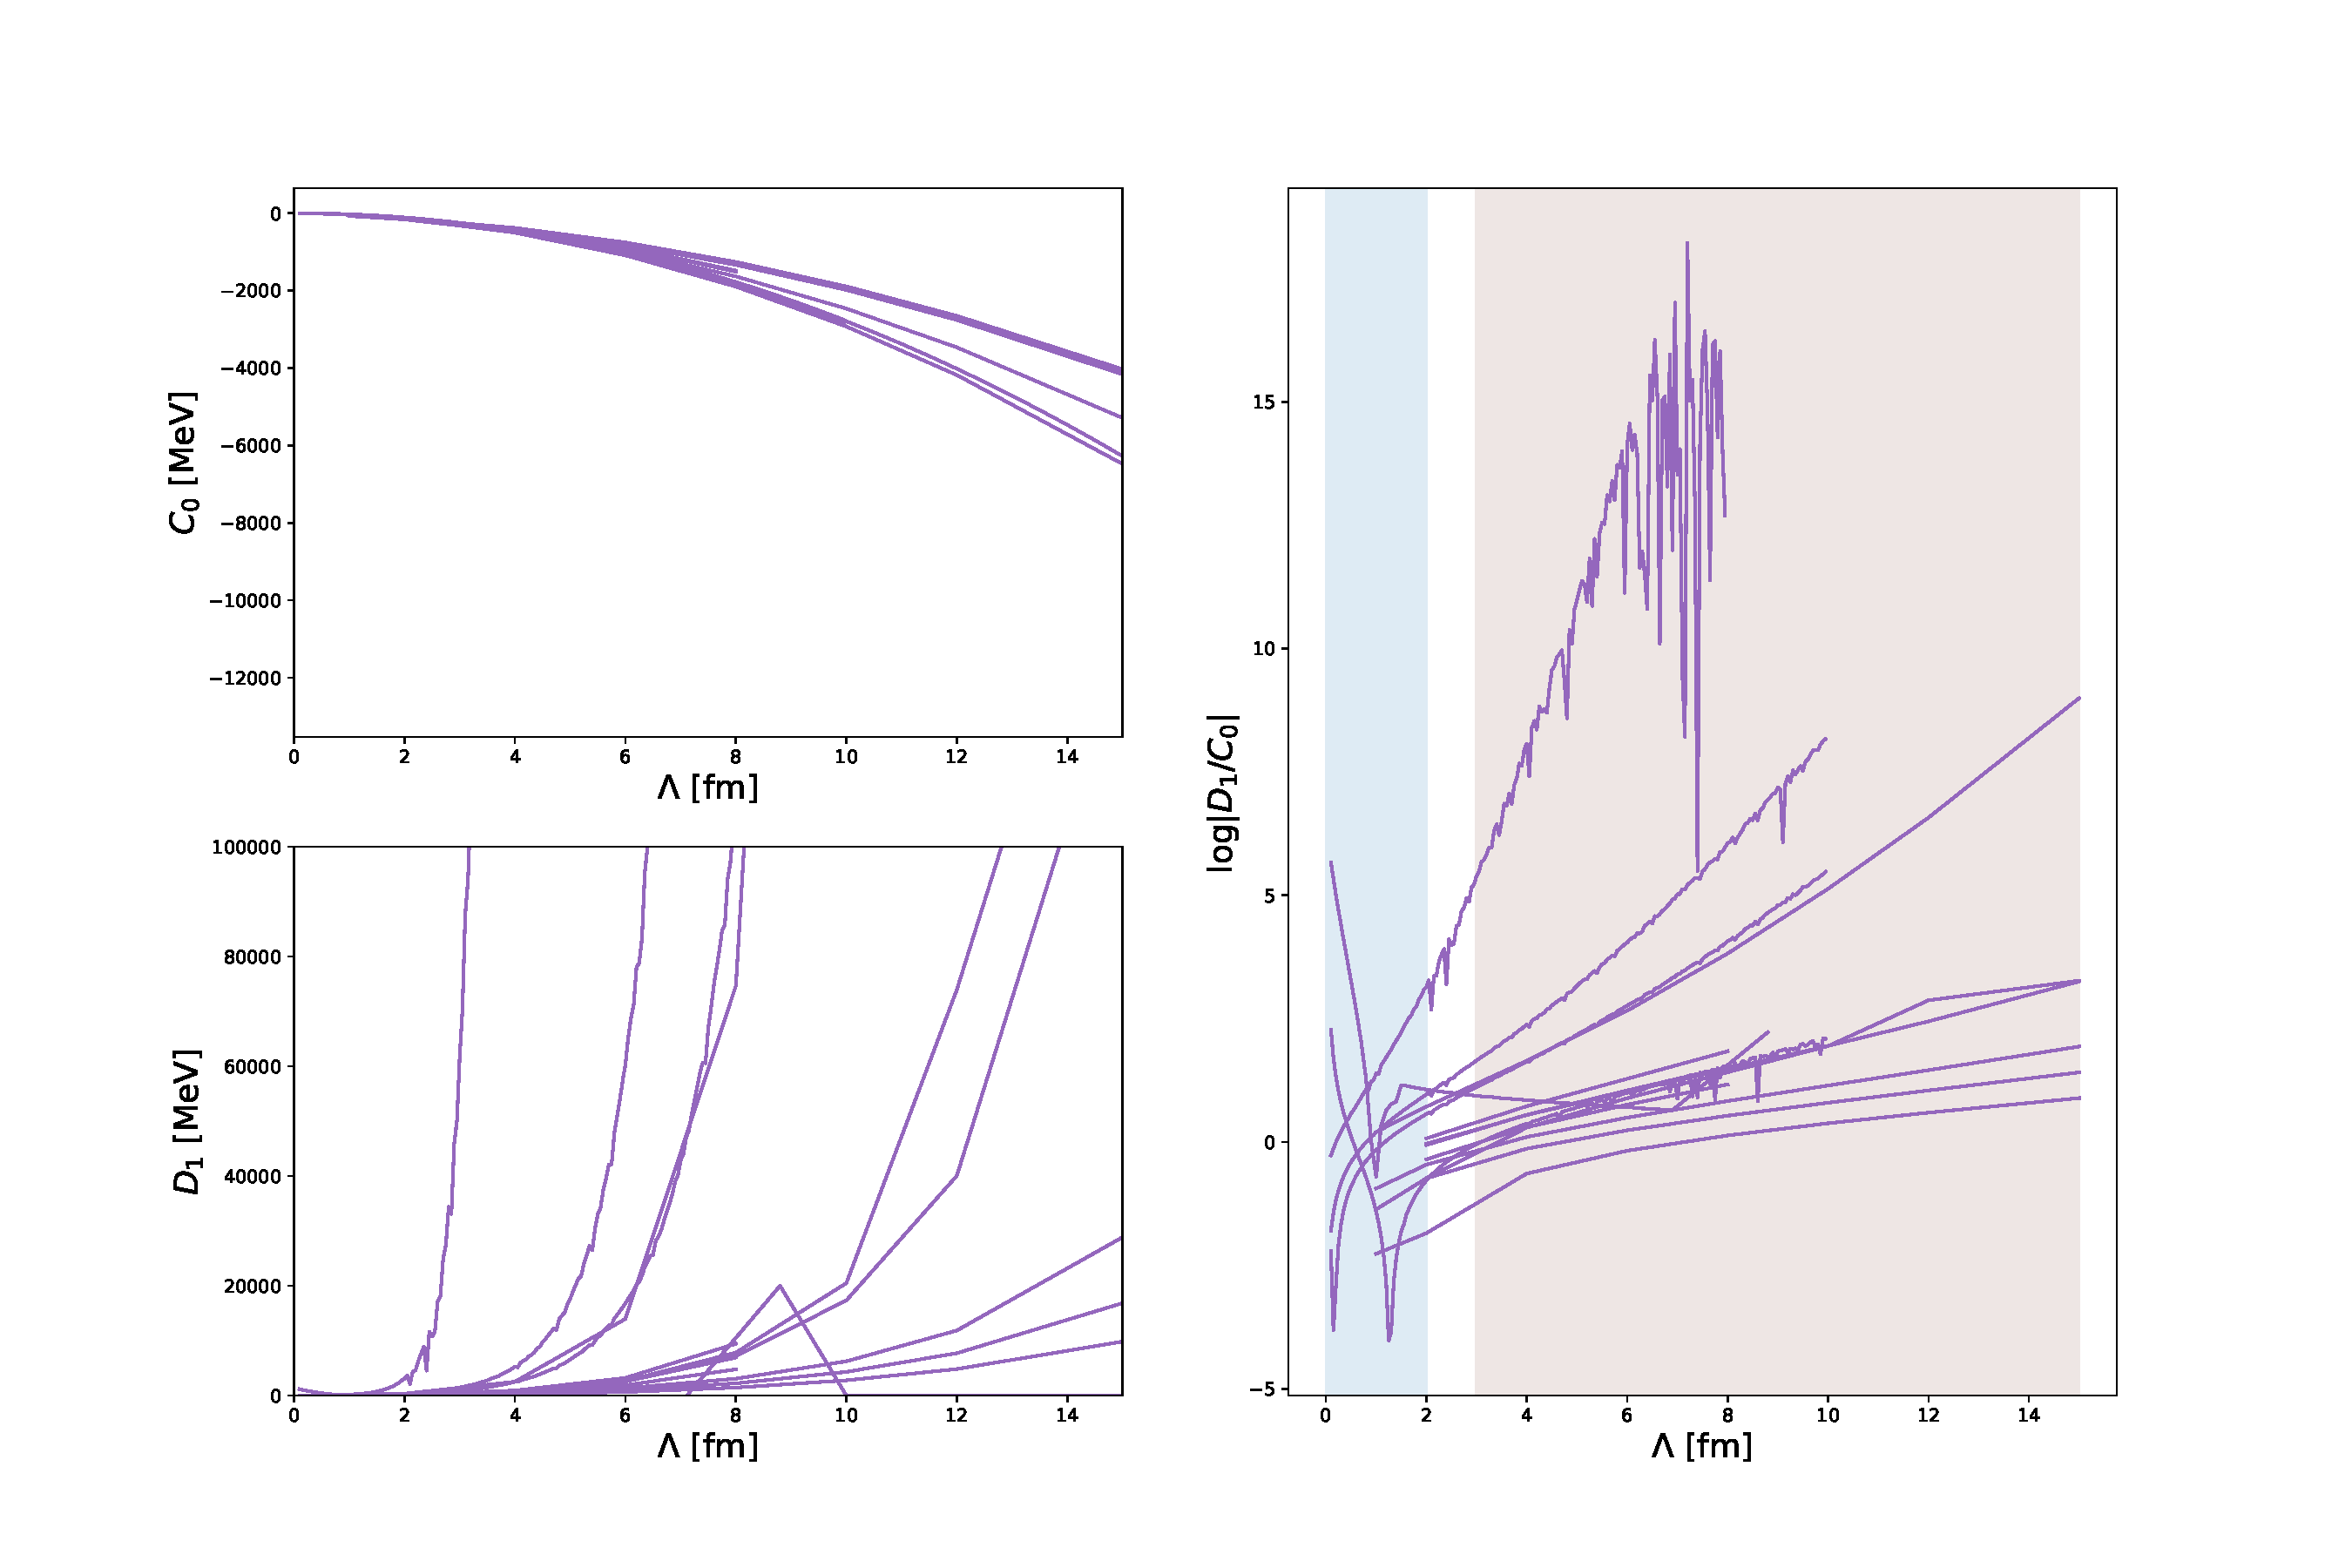
\includegraphics[width=0.95\textwidth,angle=0]{./lecsets.pdf} 
\label{fig:lecs}
\caption{Cutoff dependence of the two- and three-body interaction
 strengths, individually and relative to each other. The various
 curves. The various dependencies correspond to 
 $B(2)\in (0,20)$ and $B(3)\in (1.5,54)$ for atom masses between
$938$~MeV and $1640~$MeV. The shades roughly mark interval in which the 
three-body force is attractive (blue) or repulsive (brown).}

From \figref{fig:lecs}, we draw the following conclusions:
\begin{itemize}
\item $\dd\propto e^{\kappa\Lambda}$ for $\Lambda>$ some lower limit which
is related to $B(3)$ and is close to the point where the interaction
strength changes sign, namely, from an attractive to a repulsive force.
\item Foreseeing another bound state to enter the three-atom spectrum
once the interaction strength reaches a certain magnitude at some cutoff,
we expect this pattern to repeat itself if one identifies that newly
found pole as the one which represents the renormalization condition
for $\dd$.
\item For $B(2)\to 0$ and $B(3)\to 0$, \ie, in the multi-resonant
limit, the three-body force has a static, repulsive character. The
interaction pair is ``Janus-like'', an always attractive two-body
side and an ever repulsive three-body face. 
\end{itemize}

\end{figure}

\section{Appendix: The core wave function}
I assume that a spin-independent zero-range interaction renormalized to a shallow dimer and a shallow trimer
implies the existence of a sequence of particle-stable bosonic $A$-body states with binding energies
ordered as in
\be\la{eq:be_ordering}
0\approx B(2)\lesssim B(3)<B(4)<\ldots<B(A_\text{max})\approx B_\text{GS}(4)\;\;.
\ee
Thus, a single bound state comprises the discrete spectrum for $A<4$, while for $A\geq 4$, a pair of states emerges
with one close to the next-smaller $A+1$ threshold and the ground state relatively deep.
Further I assume that the \abb~system emerges as a pole at the $A+1$ normal branch point which marks the onset of
scattering of a single particle off the $A$-boson ground state. In some surrounding of this branch point, the amplitude
describes either elastic scattering or a two-fragment bound state. 

Our ansatz for this $A$-boson ground state
(symmetric in space \wrt particle exchange) is
\be
\phi_A:=e^{-\frac{a}{2}\sum_{i=1}^{\red{A}}\vcl{i}^2}=e^{-a\sum^{\red{A-1}}\vcl{i}^2-a\sum^{\red{A-1}}_{\red{i<j}}\vcl{i}\cdot\vcl{j}}\la{eq.wfktphi}\;\;.
\ee
Instead of single-particle coordinates, the usage of cluster coordinates identifies
the centre of mass as the origin of a ``harmonic'', effective potential, in which the
particles reside in their independent-particle/mean-field ground state. All observables
of the system in this state depend thus on a single
parameter, the (oscillator) width $a$. The root-mean-square radius, in particular, relates to
$a$ via
\begin{align}
\mathfrak{r}^2=&\frac{\int\limits_{\mathbb{R}^{3(A-1)}}d(\vcl{1},\ldots,\vcl{\red{A-1}})~
\sum_{i=1}^{\red{A-1}}\vcl{i}^2\phi_A^2}
{\int\limits_{\mathbb{R}^{3(A-1)}}d(\vcl{1},\ldots,\vcl{\red{A-1}})~\phi_A^2}\\
=&\frac{3}{2}\cdot\frac{(A-1)^2}{A}\cdot a^{-1}\stackrel{A\gg 1}{=}
\frac{3}{2}\cdot A\cdot a^{-1}\;\;.
%=&r^2_0\cdot A^{\frac{2}{3}}
\end{align}
We assume the correlation between the radius $\mathfrak{r}$ and the ground-state wave function of the
$3$-nucleon system, to hold for any spatially symmetric $A$-boson system. However, the functional
relation, $\mathfrak{r}=f\left[A,B(3),B(2)\right]$, is unknown (to the best of our knowledge).

We employ the assumption of a radius which grows almost proportional to the volume of
$A$ spheres, \ie, $\propto A^{\frac{1}{3}+\delta_V}$.
With the parameter $\delta_V$, deviations from the liquid-drop approximation are allowed,
$$
\delta_V\left\lbrace
\begin{array}{cl} >0 & \text{faster than voluminous growth}\\ 
                 <0 & \text{less than volume growth}
\end{array}\right.
$$
By ``SVM measuring'' $r_0$ for some $A$, we
implicitly relate the parameters of the theory, namely, the cutoff $\lambda$, the mass $m_N$, and
the LECs/few-body renormalization conditions to $a$.

\newpage
\section{Appendix: Inter-cluster Potential}
Consider two compound systems, whose relative motion is much slower compared with the
motion of the particles within each of these fragments. Within an arbitrarily small
time interval, the probability of a given particle to interact/hit/overlap with another
particle is then enhanced for the partner belonging to the same compound.
\[P_{dt}(\text{intra})\gg P_{dt}(\text{inter})\]
or
\[\text{\#(internal collisions)}\gg\text{\#(inter-cluster collisions)}\;\;.\]
The relative motion of particles within each cluster is then decoupled from, {\it one}, the
relative motion \wrt~the other cluster(s), {\it and two}, the internal motion
in those. In turn, the internal structure affects cluster-relative motion.
This reasoning underlies the single-channel resonating-group approximation and
also foreshadows the non-hermitian character of the effective interaction.

\begin{gather}
\cM\subd=\begin{pmatrix}4a & & & \\ & 4a & &\multicolumn{2}{l}{\!\!\!\!(2a)_\nabla}\\
 \multicolumn{2}{c}{(2a)_\triangle} & \ddots & \\ & & & & 4a \\\end{pmatrix}
\;\;;\;\;\ve{\cS}\subd =\ve{0}\;\;;\;\;B\subd =(R-R')
\end{gather}

\paragraph*{Properties of the effective \abb~potential}
Strength factors and exponents, \ie, ranges, of the effective two-body potential between an
$A$-boson bound state and a particle which is flavour- and mass-equal to one of the bosons are
listed in \tabref{tab.rgmpot}.
\begin{itemize}
\item All terms in the effective potential retain a finite range even for zero-range two- and three-body
interactions ($\Lambda\to\infty$).
\item The range of terms originating from the two-body interaction is $\approx 2\times$ as large as the one
of the terms proportional to $D_1^\Lambda$.
\item For $A\to\infty$, the interaction becomes local, \ie, $\beta\to0$.
\item For $A\gg1$, the terms $\eta_1$ and $\zeta_2$ grow linearly with $A$ consistent with the number
of pairwise interactions between the orbiter and a core constituent. The terms
$\eta_{2,3}$ and $\zeta_{3,4}$) increase in magnitude quadratically with $A$ which reflects the $(A-1)(A-2)$
possible ways triplets can be selected including the orbiter and two core particles.
\item The strength of the exchange term ($\zeta_1$) is independent of $A$ and $\Lambda$. It depends linearly
on the energy and is repulsive in even, and attractive in odd partial waves ($i^lj_l(ir)\gtrless0\;\;\forall r$ for ${\text{even}\atop\text{odd}}\;\;l$).
\end{itemize}

%\begin{table}
% 
%\centering
%\caption{\label{tab.rgmpot}{Defining parameters of the effective potential between
%a Gaussian $A$-body core, characterized via the width $a$~\eqref{eq.rgm.corewfkt},
%and one {\it odd} particle (see \eqref{eq.rgm.sglnonloc}).
%The 2- and 3-body LECs $C^\Lambda_0$ and $D^\Lambda_1$ are
%calibrated to a 2- and 3-body symmetric bound state (see table~\ref{tab.legend}).
%$A\mprime=A-1, A\mdprime=A-2, \ldots$. The coefficients $\eta_i,\zeta_i$ {\bf do}
%consider non-zero interacting pair and triplet contributions from $\sum_{i<A}$ and
%$\sum_{i<A\atop j<A-1}$ but {\bf not} $(-1)^{\mathfrak{p}}$.}}
%
%\small
\newpage

\begin{widetext}

\begin{align*}
\mathfrak{v}(\ve{R},\ve{R}')=&
\;\;\;C_0^\Lambda\cdot
\frac{8A\mprime(a A)^{3/2}}
{\left(4aA+A\mprime\Lambda^2\right)^{3/2}}&&\cdot
e^{-\frac{aA\Lambda^2}{4aA+A\mprime\Lambda^2}\ve{R}^2}&&\left(V^{(2)}_{dir}\right)\\
%
&+D_1^\Lambda\cdot
\frac{32 a^3 A\mdprime A\mprime A^{3/2}}
{\left(16 a^2 A+4 a (3 A-1) \Lambda ^2+A\mdprime \Lambda ^4\right)^{3/2}}
&&\cdot
e^{-\frac{2aA\Lambda ^2 \left(2 a +\Lambda ^2\right)}{16 a^2 A+4 a (3 A-1) \Lambda ^2+A\mdprime \Lambda ^4}\ve{R}^2}&&\left(V^{(3_a)}_{dir}\right)\\
%
&+D_1^\Lambda\cdot
\frac{32 a^3 A\mdprime A\mprime A^{3/2}}
{\left(16 a^2 A+8 a (A-1) \Lambda^2+A\mdprime \Lambda^4\right)^{3/2}}
&&\cdot e^{-\frac{2 a A \Lambda^2}{4 a A+A\mdprime \Lambda^2}\ve{R}^2}&&(V^{(3_*)}_{dir})\\
%
&&\mathclap{\hdashrule{\columnwidth}{0.4pt}{0.3em}}\\
%
&+\frac{2 \sqrt{2} (aA^3)^{3/2}}{\left(A\mprime (A+1)^2\right)^{3/2}}\cdot\widehat{\mathfrak{O}}_1
&&\cdot e^{-\frac{a \left(A^3+A\right)}{2 A\mprime (A+1)^2}\ve{R}^2-\frac{2 a A^2}{A\mprime (A+1)^2}\ve{R}\cdot\ve{R}'-\frac{a \left(A^3+A\right)}{2 A\mprime (A+1)^2}\ve{R}'^2}&&\left(V^{(\mathbb{1})}_{Ex}\right)\\
%
&&\mathclap{\hdashrule{\columnwidth}{0.4pt}{0.3em}}\\
%
&+C_0^\Lambda\cdot
\frac{8\pi^{-3/2} (A+1)^{-3} A\mprime (a A)^{9/2}}
{\left(4 a^2 A\mprime+aA\mdprime \Lambda ^2\right)^{3/2}}
&&\cdot e^{-\frac{a A \left(4 a \left(A^2+1\right)+\left(3 A^2+A+2\right) \Lambda ^2\right)}{2 (A+1)^2 \left(4 a A\mprime+A\mdprime \Lambda ^2\right)}\ve{R}^2}\\
&&&\cdot e^{-\frac{4a A^2 \left(2 a+\Lambda ^2\right)}{(A+1)^2 \left(4 a A\mprime+A\mdprime \Lambda ^2\right)}\ve{R}\cdot\ve{R}'}\\
&&&\cdot e^{-\frac{a A \left(4 a \left(A^2+1\right)+\left(A^2-A+2\right) \Lambda ^2\right)}{2 (A+1)^2 \left(4 a A\mprime+A\mdprime \Lambda ^2\right)}\ve{R}'^2}&&\left(V^{(2)}_{Ex}\right)\\
%
&+D_1^\Lambda\cdot
\frac{32 \pi^{-\frac{3}{2}} (A+1)^{-3} A\mdprime A\mprime (a A)^{9/2}}
{\left(16 a^2 A\mprime+4 a (3 A-4) \Lambda ^2+A\mtprime \Lambda ^4\right)^{3/2}}
&&\cdot e^{-\frac{a A \left(16 a^2 \left(A^2+1\right)+4 a \left(5 A^2+A+4\right) \Lambda ^2+\left(5 A^2+2 A+3\right) \Lambda ^4\right)}{2 (A+1)^2 \left(16 a^2 A\mprime+4 a (3 A-4) \Lambda ^2+A\mtprime \Lambda ^4\right)}\ve{R}^2}\\
&&&\cdot e^{-\frac{2 a A^2 \left(16 a^2+16 a \Lambda ^2+3 \Lambda ^4\right)}{(A+1)^2 \left(16 a^2 A\mprime+4 a (3 A-4) \Lambda ^2+A\mtprime \Lambda ^4\right)}\ve{R}\cdot\ve{R}'}\\
&&&\cdot e^{-\frac{a A \left(16 a^2 \left(A^2+1\right)+4 a \left(3 A^2-A+4\right) \Lambda ^2+\left(A^2-2 A+3\right) \Lambda ^4\right)}{2 (A+1)^2 \left(16 a^2 A\mprime+4 a (3 A-4) \Lambda ^2+A\mtprime \Lambda ^4\right)}\ve{R}'^2}&&\left(V^{(3_a)}_{Ex}\right)\\
&+D_1^\Lambda\cdot
\frac{32 \pi^{-\frac{3}{2}} (A+1)^{-3} A\mdprime A\mprime (a A)^{9/2}}
{\left(16 a^2 A\mprime+4 a (2A-4) \Lambda ^2+A\mtprime \Lambda ^4\right)^{3/2}}
&&\cdot e^{-\frac{a A \left(4 a \left(A^2+1\right)+\left(5 A^2+2 A+3\right) \Lambda ^2\right)}{2 (A+1)^2 \left(4 a A\mprime+A\mtprime \Lambda ^2\right)}\ve{R}^2}\\
&&&\cdot e^{-\frac{2 a A^2 \left(4 a+3 \Lambda ^2\right)}{(A+1)^2 \left(4 a A\mprime+A\mtprime \Lambda ^2\right)}\ve{R}\cdot\ve{R}'}\\
&&&\cdot e^{-\frac{a A \left(4 a \left(A^2+1\right)+\left(A^2-2 A+3\right) \Lambda ^2\right)}{2 (A+1)^2 \left(4 a A\mprime+A\mtprime \Lambda ^2\right)}\ve{R}'^2}&&\left(V^{(3_*)}_{Ex}\right)\\
\end{align*}
\end{widetext}
%
The strengths of the exchange-interaction terms for $A\gg 1$ and/or $\Lambda\gg 1$\fm is then related to the corresponding
direct-interaction strength via
\be
\zeta_{n+1}=\eta_n\cdot\left(\frac{A}{A+1}\right)^3\left(\frac{a}{\pi}\right)^{3/2}\;\;\;.
\ee
The fraction $\left(\frac{a}{\pi}\right)^{3/2}$ is the inverse of an integration of the non-local
terms assuming a constant wave function (exponents scale with $a$ which produces an $\sqrt{\pi/a}$ upon integration,
and the spherical Bessel functions provide the remaining $a^{-1}$).

In order to study the zero-range limit and the related renormalization-group invariance, the large $\Lambda$
behaviour is of interest. In this limit, the potential scales as
%
\begin{widetext}
\begin{align*}
\lim_{\Lambda\to\infty}\mathfrak{v}(\ve{R},\ve{R}')=&\;\;\;\;\;\mathcal{O}(A)\cdot\frac{C_0^\Lambda}{\Lambda^3}\cdot a^{\frac{3}{2}}\cdot e^{-a\ve{R}^2}
&&+2\cdot\mathcal{O}(A^2)\cdot \frac{D_1^\Lambda}{\Lambda^6}\cdot a^3\cdot e^{-2a\ve{R}^2}\\
&+\mathcal{O}(A)\cdot\frac{C_0^\Lambda}{\Lambda^3}\cdot a^{3}\cdot e^{-\frac{3}{2}a\ve{R}^2-\frac{4a}{\mathcal{O}(A)}\ve{R}\cdot\ve{R}'-\frac{3}{2}a\ve{R}'^2}
&&+2\cdot\mathcal{O}(A^2)\cdot\frac{D_1^\Lambda}{\Lambda^6}\cdot a^{\frac{9}{2}}\cdot e^{-\frac{5}{2}a\ve{R}^2-\frac{6a}{\mathcal{O}(A)}\ve{R}\cdot\ve{R}'-\frac{5}{2}a\ve{R}'^2}\\
&+\mathcal{O}(1)\cdot a^{\frac{3}{2}}\cdot e^{-\frac{a}{2}\ve{R}^2-2a\ve{R}\cdot\ve{R}'-\frac{a}{2}\ve{R}'^2}\;\;\;,&&\\
\end{align*}
\end{widetext}
and terms were organized their origin from pair or triplet interactions. The third-row term stems from the norm-exchange
kernel. This skeleton of the potential is now fed into the partial-wave projected RGM equation \eqref{eq.rgm.sglnonloc.pw}
to yield
%
\begin{widetext}
\begin{subequations}\la{eq.rgm.pw}
\begin{gather}
\int\Bigg\lbrace\frac{\hbar^2}{2\mu}\left[-\partial^2_R\left(\mathbb{1}+(\mathfrak{o}_E\leftrightarrow\mathfrak{o}_\mu)\right)+
\frac{l(l+1)}{R^2}\left(\mathbb{1}+(\mathfrak{o}_E\leftrightarrow\mathfrak{o}_L)\right)\right]
\phi_{lm}(R\mprime)\la{eq.rgm.pw.a}\\
%
-E\left(\delta(R-R\mprime)+(-)^{l+1}\mathfrak{o}_E(1)\left(\frac{a}{\pi}\right)^{3/2}
e^{+\frac{1}{2}\mathfrak{o}_E(aA^{-1})RR\mprime-\frac{1}{2}\mathfrak{o}_E(a)\ve{R}^2-\frac{1}{2}\mathfrak{o}_E(a)\ve{R}'^2}\right)\la{eq.rgm.pw.b}\\
%
+\mathfrak{o}_2(A)\cdot\frac{C_0^\Lambda}{\Lambda^3}\cdot a^{\frac{3}{2}}\cdot
e^{-\mathfrak{o}_2(a)\ve{R}^2}
\left(\delta(R-R\mprime)+(-)^{l+1}\mathfrak{o}_2(1)\left(\frac{a}{\pi}\right)^{3/2}
e^{+\mathfrak{o}_2(aA^{-1})RR\mprime-\mathfrak{o}_2(a)\ve{R}'^2}\right)\la{eq.rgm.pw.c}\\
%
+2\cdot\mathfrak{o}_3(A^2)\cdot\frac{D_1^\Lambda}{\Lambda^6}\cdot a^{3}\cdot
e^{-2\mathfrak{o}_3(a)\ve{R}^2}
\left(\delta(R-R\mprime)+(-)^{l+1}\mathfrak{o}_3(1)\left(\frac{a}{\pi}\right)^{3/2}
e^{+2\mathfrak{o}_3(aA^{-1})RR\mprime-2\mathfrak{o}_3(a)\ve{R}'^2}\right)
\Bigg\rbrace\phi_{lm}(R\mprime)dR\mprime\la{eq.rgm.pw.d}\\
 =0\;\;\;.\nonumber
\end{gather}
\end{subequations}
\end{widetext}
%
The first and second row of this equation demonstrate the effect of the antisymmetrization on the single-particle
characteristics of the system which is solely the reduced mass. For even partial waves, the exchange of the particle
amounts to an increased mass if the particle is close to the core, while for a large separation the original
mass dictates the free propagation. The distance over which the mass is significantly enlarged is set by the
core size $a$ in the exponent of \eqref{eq.rgm.pw.b}. The mass/kinetic-energy correction due to exchange is thus
characterized repulsive or attractive solely by the partial wave (only one single permutation comprises the 
antisymmetrization) with strength and range increasing with the size of the core.

The exchange has qualitatively the same effect on the terms associated with the two- and three-body contact interactions.
Corrections to both \eqref{eq.rgm.pw.c} and \eqref{eq.rgm.pw.d} increase (odd) or decrease (even) the interaction
strength without changing its attractive or repulsive character. Exchange effects do not turn an attractive interaction
repulsive or vice versa. A potential destabilization is thus driven by a weakening of an otherwise sufficiently attractive 
direct interaction in combination with a genuine but interaction-independent repulsion as emergent from the
kinetic part of the system. This insight in combination with the strengths of the interaction being
much larger in magnitude for $\lim_{\Lambda\to\infty}$ compared with the kinetic-energy factors justify our qualitative
conjectures in the discussion of \figref{fig:RGM2} which were based on the local approximation.
%2   & $
%\to\frac{1}{2}a
%\to \mathcal{O}(1)\cdot a^{\frac{3}{2}}
%\toinf\mathcal{O}(A)\cdot \frac{C_0^\Lambda}{\Lambda^3}\cdot a^{\frac{3}{2}} e^{-\frac{A}{A-1}\cdot a}
%\toinf\mathcal{O}(A^2)\cdot \frac{D_1^\Lambda}{\Lambda^6}\cdot a^3
%\toinf\frac{A}{A-2}\cdot 2a
%3 & 
%\toinf\mathcal{O}(A^2)\cdot \frac{D_1^\Lambda}{\Lambda^6}\cdot a^3$ & $
%\toinf\frac{A}{A-2}\cdot 2a$ \\
%\hline
%\to\frac{1}{2}a
%\to\mathcal{O}(A^{-1})\cdot 2a
%2 & 
%\toinf\mathcal{O}(A)\cdot \frac{C_0^\Lambda}{\Lambda^3}\cdot a^3$ & 
%\toinf \frac{3}{2}a$&
%\toinf \mathcal{O}(A^{-1})\cdot4a$&
%3 &
%\toinf\mathcal{O}(A^2)\cdot \frac{D_1^\Lambda}{\Lambda^6}\cdot a^{\frac{9}{2}}$&
%\toinf \frac{5}{2}a$&
%\toinf \mathcal{O}(A^{-1})\cdot6a$&
%4 &
%\toinf\mathcal{O}(A^2)\cdot \frac{D_1^\Lambda}{\Lambda^6}\cdot a^{\frac{9}{2}}$&
%\toinf \frac{5}{2}a$&
%\toinf \mathcal{O}(A^{-1})\cdot6a$&
%\end{table}
\bibliographystyle{unsrt}
\bibliography{Thebibliography.bib}
\end{document}
